\documentclass{article}
\usepackage{tikz}

\begin{document}
  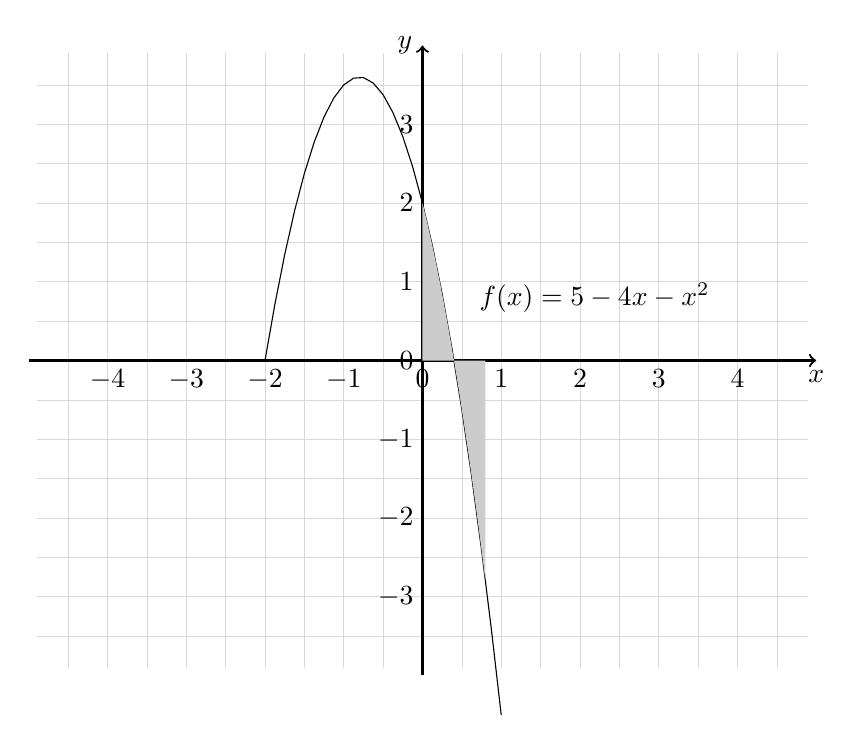
\begin{tikzpicture}
    \draw[very thin, gray!30, step=0.5 cm](-4.9,-3.9) grid (4.9,3.9);

   
    \draw [thick] [->] (-5,0)--(5,0) node[right, below] {$x$};
     \foreach \x in {-4,...,4}
       \draw[xshift=\x cm, thick] (0pt,-0.5pt)--(0pt,0.5pt) node[below] {$\x$};

    \draw [thick] [->] (0,-4)--(0,4) node[above, left] {$y$};
     \foreach \y in {-3,...,3}
       \draw[yshift=\y cm, thick] (-0.5pt,0pt)--(0.5pt,0pt) node[left] {$\y$};

    \draw [scale=0.4,domain=-5:2.5, variable=\x]
      plot ({\x}, {5-4*\x-\x*\x}) node[right] at (1.5,2) {$f(x)=5-4x- x^2$};


 \fill [gray!40, scale=0.4,domain=0:2, variable=\x]
      (0, 0)
      -- plot ({\x}, {5-4*\x-\x*\x})
      -- (2, 0)
      -- cycle;

  \end{tikzpicture}
\end{document}
